\subsection{Inverting Zero-Crossing Level Detector With Hysteresis:}

For the circuit in Figure 3.3.0 we simulate it and captured the results in Figures 4.3.0, 4.3.1 and 4.3.2:

\begin{figure}[H]
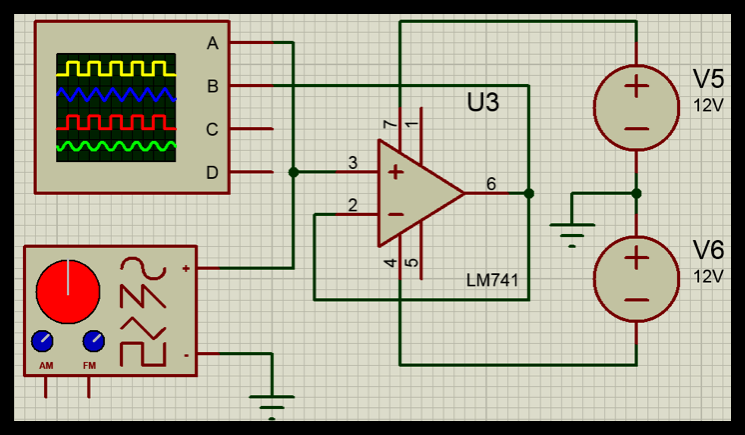
\includegraphics[width = 16.5cm, height = 6cm]{s3.png}
\centering \linebreak \linebreak Figure 4.3.0: Inverting zero-crossing circuit.
\end{figure} \hfill

\begin{multicols}{2}
\begin{figure}[H]
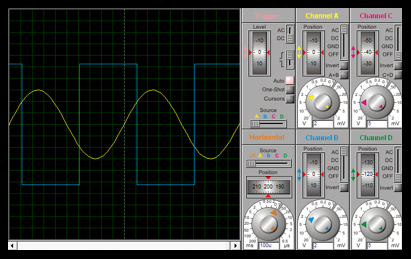
\includegraphics[width = 8cm, height = 5cm]{s3-2.png}
\centering \linebreak \linebreak Figure 4.3.1: Input and output waveform.
\end{figure} \hfill

\begin{figure}[H]
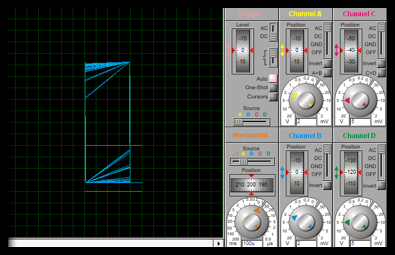
\includegraphics[width = 8cm, height = 5cm]{s3-3.png}
\centering \linebreak \linebreak Figure 4.3.2: Transfer function for Figure 4.3.0.
\end{figure} \hfill
\end{multicols} 

\pagebreak